\normaltrue
\correctionfalse

%\UPSTIidClasse{11} % 11 sup, 12 spé
%\newcommand{\UPSTIidClasse}{12}


\exer{Mouvement TT -- $\star$ \label{STAT:02:B2:13:03:02}}
\setcounter{question}{0}\marginnote{\xpComp{STAT}{03}}%\UPSTIcompetence{B2-13}
\index{Compétence STAT-03}
\index{Mécanisme à 2 translations}
\ifcorrection
\else
\marginnote{\textbf{Pas de corrigé pour cet exercice.}}
\fi

\ifprof
\else
Soit le mécanisme suivant. On note $\vect{AB}=\lambda(t)\vect{i_0}$ et $\vect{BC}=\mu(t)\vect{j_0}$.
\begin{marginfigure}
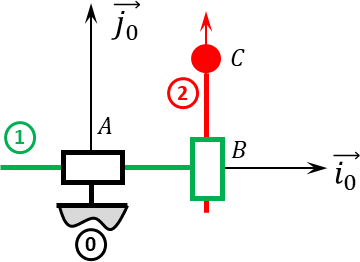
\includegraphics[width=\linewidth]{03_TT_01}
\end{marginfigure}
\fi

\question{Déterminer $\vectv{C}{2}{0}$ par dérivation vectorielle ou par composition.}
\ifprof
\else
\fi

\question{Donner le torseur cinématique $\torseurcin{V}{2}{0}$ au point $C$.}
\ifprof
\else
\fi

\question{Déterminer $\vectg{C}{2}{0}$.}
\ifprof
\else
\fi

\ifprof
\else
\marginnote{Corrigé voir \ref{STAT:02:B2:13:03:02}.}
\fi


